\documentclass[11pt,a4paper]{article}
\usepackage[T1]{fontenc}
\usepackage[utf8]{inputenc}
\usepackage{lmodern,microtype}
\usepackage[margin=22mm,headheight=14pt]{geometry}
\usepackage{graphicx,booktabs,tabularx,array,amsmath,enumitem,float}
\usepackage{xcolor,tikz,caption,fancyhdr,titlesec}
\usetikzlibrary{arrows.meta,positioning,fit,calc}
\definecolor{navy}{HTML}{183850}
\definecolor{lightblue}{HTML}{EDF3F7}
\definecolor{muted}{HTML}{526575}
\usepackage[colorlinks=true,linkcolor=navy,citecolor=navy,urlcolor=navy]{hyperref}
\hypersetup{pdftitle={VisuAlgo+ — CA Report Draft},pdfauthor={Truong Van Quoc Bao}}
\setlength{\parindent}{0pt}
\setlength{\parskip}{6pt}
\linespread{1.06}
\setlist{nosep,leftmargin=1.6em}
\setlength{\emergencystretch}{2em}
\renewcommand{\arraystretch}{1.18}
\titleformat{\section}{\Large\bfseries\color{navy}}{\thesection}{.65em}{}
\titleformat{\subsection}{\large\bfseries\color{navy}}{\thesubsection}{.65em}{}
\titlespacing*{\section}{0pt}{0pt}{10pt}
\titlespacing*{\subsection}{0pt}{12pt}{4pt}
\captionsetup{font=small,labelfont=bf,skip=5pt}
\pagestyle{fancy}\fancyhf{}
\fancyhead[L]{\small\color{muted}VisuAlgo+}
\fancyhead[R]{\small\color{muted}CP4101 CA Report \textbar\ Draft}
\fancyfoot[C]{\small\thepage}
\renewcommand{\headrulewidth}{.3pt}
\newcommand{\code}[1]{\texttt{#1}}
\newcommand{\shot}[4]{\begin{figure}[tbp]\centering\includegraphics[width=#2\linewidth]{figures/#1}\caption{#3}\label{#4}\end{figure}}
\newcommand{\page}{\par\vspace{8pt}}
\begin{document}
\begin{titlepage}
\centering
{\large NATIONAL UNIVERSITY OF SINGAPORE\\School of Computing\par}
\vspace{22mm}
{\Huge\bfseries\color{navy}VisuAlgo+\par}
\vspace{5mm}
{\LARGE Rebuilding Interactive\\Algorithm Visualizations\par}
\vspace{10mm}
{\Large CP4101 Final Year Project\\Continuous Assessment Report\par}
\vspace{12mm}
{\large Truong Van Quoc Bao\\A0276275U\par}
\vspace{7mm}
{Supervisor: A/P Steven Halim\\Academic Year 2026/27, Semester 1\\4 November 2026\par}
\vspace{9mm}
{\small\bfseries DRAFT FOR REVIEW\par}
\vspace{5mm}
\begin{minipage}{.94\textwidth}
\textbf{Abstract.} VisuAlgo+ is a collaborative project to rebuild VisuAlgo with a renewed technical foundation and a redesigned interface while preserving its educational purpose. My work focuses on the visualization and interaction layer: graph, tree and sorting visualizers, their editing and playback behaviour, and their integration into a common interface. The work began with standalone prototypes and progressed to a single application using a shared panel layout. This report explains the separation of input, layout and playback state; the V10 panel-group model; algorithm extensions and their validation; and short explanations placed on the drawing. The audited application contains 11 graph algorithm identifiers, seven tree workspaces and eight sorting algorithms. Its recorded validation on 1 November 2026 reports 3,273 passing unit tests and 151 passing browser cases. These results support functional progress. A Week 10 user trial provided formative feedback and recorded interactions that informed subsequent UI/UX refinements, including floating text on the canvas. Neither source establishes improved learning outcomes or comparative usability. The next phase will strengthen interaction testing, evaluate representative learning tasks and investigate a limited integration with the separate WebAssembly engine.
\end{minipage}
\vfill
{\small Application snapshot: \code{662e7b3}\quad\textbar\quad Evidence snapshot: \code{67ce56c}\par}
\end{titlepage}
\setcounter{page}{2}

\begingroup
\setlength{\parskip}{4pt}
\linespread{1.0}\selectfont
\section{Introduction and Objectives}
\subsection{Project background}
VisuAlgo provides interactive visualizations of data structures and algorithms. Its original design brings different topics into a consistent environment and allows students to explore their own inputs~\cite{halim2012}. These strengths are the starting point for VisuAlgo+.

In an early discussion, A/P Steven Halim described the existing Laravel/PHP, MySQL, D3 and jQuery stack and encouraged us to explore a modern foundation for both the interface and execution engine. This background reflects my account of that discussion~\cite{evidence}. The rebuild retains useful technologies, including D3 for selected layout and animation tasks.

The aim is a modern successor that preserves VisuAlgo's educational purpose and useful interactions while supporting future development. The current deliverable is an experimental application, not yet a full replacement.

\subsection{Personal motivation and role}
My motivation for joining VisuAlgo+ comes from my background in competitive programming and teaching. Participating in many programming competitions and achieving strong results has given me substantial experience with algorithms and data structures. Teaching students passionate about competitive programming has helped me explain these concepts from different perspectives and recognize where learners need clarification.

I hope to apply both experiences to VisuAlgo+'s user interface and user experience, helping learners follow why an algorithm makes a decision, how its state changes, and how those changes produce the result. This perspective guides which intermediate states I show, how I connect drawings with pseudocode, and where short explanations could clarify a step.

My initial responsibility is the visualization and interaction layer for graph algorithms, tree-based data structures and sorting algorithms. This includes developing the visualizers, supporting input editing and step-by-step playback, and integrating them into a consistent interface. Working with Kerk on the shared design and integration, I aim to turn my algorithmic knowledge and teaching experience into practical improvements that can later be evaluated with learners.

\subsection{Objectives and current scope}
The project has five working objectives:
\begin{enumerate}
\item Select suitable modern and widely adopted technologies for rebuilding the platform.
\item Preserve useful algorithm exploration, input editing and step-by-step explanation from VisuAlgo.
\item Provide a consistent interface across different algorithm and data-structure modules.
\item Establish clear boundaries for extending visualizers and integrating execution engines.
\item Validate the rebuilt functionality and identify what still requires technical and user evaluation.
\end{enumerate}

Kerk Tai Heng, a fellow FYP student under the same supervisor, works on the engine/WASM foundation, website design system and shared infrastructure. Section~\ref{sec:approach} details our contributions and collaboration.

The current application targets desktop and laptop use. It runs TypeScript algorithm implementations in the browser. The separate WebAssembly engine has not been connected to these visualizers. Mobile design, complete feature parity with VisuAlgo and measured learning improvement are outside the completed work reported here.

\endgroup
\page
\section{Background and Related Work}
\subsection{Algorithm visualization and educational use}
Halim et al.~\cite{halim2012} present VisuAlgo as a unified web-based environment for learning algorithms. Support for user-defined inputs and consistent interaction across topics is particularly relevant to this project. A reconstruction should preserve these properties even when the rendering technology and page layout change. Reusing familiar examples and algorithm operations also provides a useful reference when checking the rebuilt functionality.

However, a working animation is not sufficient evidence of learning benefit. Hundhausen, Douglas and Stasko's meta-study of 24 studies~\cite{hundhausen2002} found that how learners used algorithm visualizations mattered more than their graphical characteristics alone. This motivates a distinction between two questions in VisuAlgo+: whether the software behaves correctly, and whether students can use it to understand and explain an algorithm. The present tests primarily address the first question. The Week 10 trial provided initial formative input; a more structured follow-up is proposed for the second.

OpenDSA combines visualizations with explanatory material, interactive exercises and proficiency assessment~\cite{opendsa}. It illustrates how visualization can form one part of a wider learning activity. VisuAlgo+ currently concentrates on exploration: editing inputs, stepping through execution, following pseudocode and inspecting state. It does not yet provide an equivalent assessed learning sequence. Therefore, the current contribution should be judged as a visualization foundation rather than a complete instructional system.

\subsection{Reusable platforms and implementation choices}
Shaffer et al.~\cite{shaffer2010} survey the algorithm-visualization field and discuss issues including availability, quality and topic coverage. Their historical survey helps motivate attention to maintainable implementations and reusable interaction patterns.

For the technical foundation, React Flow supplies an interactive node-and-edge canvas~\cite{reactflow}. The project builds algorithm-specific state, edge identities and presentation rules above that canvas. D3 supplies narrower computational tools: force simulation for graph positions and a hierarchy layout for trees~\cite{d3}. This combination separates the computation of positions from the ownership of application state. Sorting uses Canvas 2D because its main representation is an array of bars rather than an editable graph.

\subsection{Position of this work}
The project applies established algorithm, rendering and interface ideas to a practical rebuild. Its current value lies in connecting them coherently: a stable editable document, reproducible playback, shared page controls, and explanations tied to individual algorithm steps. Dockable panels and low-link algorithms are not claimed as new research techniques.

Three design questions guide the work. First, how can editing and playback share one canvas without accidentally invalidating or corrupting an execution? Second, how can different topics share a layout while preserving their own interactions? Third, how can a step remain understandable when it changes internal state but produces little visible motion? Sections~\ref{sec:state}--\ref{sec:notes} describe the implemented responses.

\page
\section{Development Approach and Responsibilities}\label{sec:approach}
\subsection{From standalone prototypes to one application}
The first stage explored interaction behaviour in standalone repositories. Graph Visualizer V1 began on 28 July; Graph Visualizer V2 followed in August with a clearer separation of document, layout and playback state. Sorting and tree prototypes explored different representations and operation models. This work provided a functional base before integration with the shared website.

During September and October, I adapted these visualizers to Kerk's design system. Kerk conducted a user survey to inform the choice between the V2 split-rail and V7 dock-based layouts. We also implemented both variants with comparable visualization functionality, allowing us to explore their interaction patterns in a working application. Following the survey and implementation work, Kerk, our supervisor and I agreed on V10 as a combined design adapted from V2 and V7, retaining selected strengths of each.



A formative user trial of V10 in Week 10 (Section 6.1) informed later refinements, including floating text. On 18 October, Kerk consolidated the separate site and visualizer copies into one application and moved common code into a shared layer. Subsequent work extended algorithms, added step notes and resolved defects found in review. Table~\ref{tab:timeline} summarizes these stages~\cite{evidence,architecture}.

\begin{table}[tbp]\small\centering
\caption{Main development stages. Dates describe recorded work, not formal assessment weeks.}\label{tab:timeline}
\begin{tabularx}{\linewidth}{@{}p{27mm}X@{}}\toprule
Period & Main outcome\\\midrule
Late July--August & Initial graph prototype, graph V2 state architecture, and standalone sorting prototype.\\
September & Tree workspaces; adaptation to V2/V7; shared website integration; separate engine-boundary experiment.\\
Early--mid October & Additional operations, playback refinements, and V10 panel-group model.\\
18--31 October & One-app consolidation; graph extensions; shared step notes; review and regression fixes.\\
\bottomrule
\end{tabularx}
\end{table}

\subsection{Individual contribution and collaboration}
My principal contributions are the standalone visualizer foundations, their integration, the core V10 layout model, algorithm and operation extensions, and the shared step-note behaviour. The first 26 recorded V10 choices were my decisions. Later choices 27--48 and the subsequent ``V10 wins'' changes were joint decisions, with Kerk implementing the associated changes. Kerk also owns the original design system, engine foundation, infrastructure and application consolidation.

I used Claude and Codex for implementation, debugging, test generation and review under my requirements and design choices. My acceptance workflow included reading changes, running the application and using tests or CI results. In late-October review sessions, Codex identified findings, Claude reproduced findings, and I selected the fixes to pursue. AI also assisted in organizing evidence and drafting this report. Such assistance is part of the development process; generated code and passing tests still require critical review, and do not establish correctness by themselves.

\page
\section{System Design and Implementation}
\subsection{Architecture of the current application}
The current build is one React and TypeScript single-page application assembled with Vite. The site layer owns routing, the top bar and the theme. A module page hosts the graph, tree or sorting visualizer. Each visualizer owns its data, algorithm execution and playback state, while shared components provide common layout and presentation utilities~\cite{architecture}.

\begin{figure}[tbp]\centering
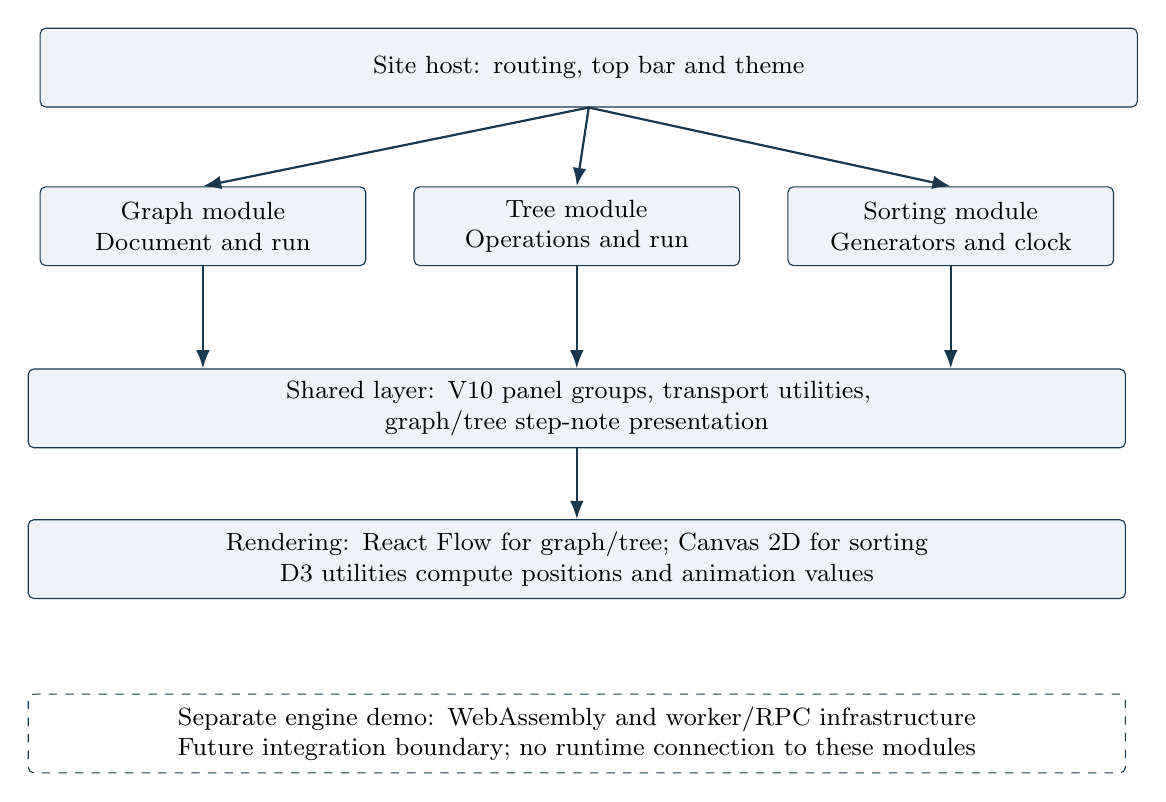
\begin{tikzpicture}[font=\small,>=Latex,
 box/.style={draw=navy,rounded corners=2pt,fill=lightblue,align=center,minimum height=10mm,text width=39mm},
 wide/.style={box,text width=137mm}, arr/.style={->,thick,draw=navy}]
\node[wide] (host) {Site host: routing, top bar and theme};
\node[box,below=10mm of host,xshift=-49mm] (g) {Graph module\\Document and run};
\node[box,right=6mm of g] (t) {Tree module\\Operations and run};
\node[box,right=6mm of t] (s) {Sorting module\\Generators and clock};
\draw[arr] (host.south) -- (g.north);\draw[arr] (host.south) -- (t.north);\draw[arr] (host.south) -- (s.north);
\node[wide,below=13mm of t] (shared) {Shared layer: V10 panel groups, transport utilities,\\graph/tree step-note presentation};
\draw[arr] (g.south) -- (shared.north -| g.south);
\draw[arr] (t.south) -- (shared.north);
\draw[arr] (s.south) -- (shared.north -| s.south);
\node[wide,below=9mm of shared] (render) {Rendering: React Flow for graph/tree; Canvas 2D for sorting\\D3 utilities compute positions and animation values};
\draw[arr] (shared) -- (render);
\node[wide,below=12mm of render,fill=white,dashed] (wasm) {Separate engine demo: WebAssembly and worker/RPC infrastructure\\Future integration boundary; no runtime connection to these modules};
\end{tikzpicture}
\caption{Current application boundaries. The lower dashed box is a separate prototype, not a dependency of the visualization application.}\label{fig:arch}
\end{figure}

This organization avoids making the shared shell responsible for algorithm logic. For example, the shell positions a Status panel, but the active algorithm determines its content. Similarly, the site can change a theme without taking ownership of a graph run. State is held in the browser; saved layout preferences use local storage.

\page
\subsection{State ownership and reproducible playback}\label{sec:state}
The graph foundation separates four concerns (Table~\ref{tab:state}). A persistent canvas is reused for editing and execution. Starting a run derives a sequence of typed steps from the current document; stepping through that sequence derives the visible presentation. This reduces the risk of keeping a separate editing graph and animation graph that gradually disagree~\cite{architecture}.

\begin{table}[tbp]\small\centering
\caption{State separation in the graph visualizer.}\label{tab:state}
\begin{tabularx}{\linewidth}{@{}p{31mm}X X@{}}\toprule
State owner & Responsibility & Example consequence\\\midrule
Graph document & Vertices, edges, weights, stable identities and topology revision. & A semantic edit invalidates the previous run.\\
Graph layout & Positions and pinned vertices. & Dragging a vertex changes the drawing without changing the algorithm input.\\
Run session & Step sequence, current index, run identity and playback status. & An outdated timer event cannot advance a newer run.\\
Presentation & Highlights, badges and derived edge/node styles. & Rewinding restores the presentation of the selected step.\\\bottomrule
\end{tabularx}
\end{table}

For example, moving vertex B should not change a shortest-path computation. Changing an edge weight should. Keeping position data separate from semantic input makes this distinction explicit. A run identity also protects against asynchronous playback events that arrive after the user stops or replaces a run.

Graph and tree algorithms build their complete step sequence when a run starts. The session then moves between idle, paused, playing and finished states. Each selected step supplies consistent information for the drawing, pseudocode highlight and status text. This eager approach makes backward stepping and seeking straightforward, but increases startup time and memory use for long runs. These costs have not yet been benchmarked.

Tree operations add a distinction between a preview and a committed document. An insertion or deletion can be explored through intermediate states before its final result is applied. This lets the learner inspect an operation without treating every animation frame as a permanent edit. Clear Apply behaviour is therefore part of the interaction model, not just a rendering detail.

\subsection{Sorting uses a different execution model}
Sorting produces operations from generators. A shared clock advances one, two or four panes, each with its own operation stream. The implementation retains executed history, buffers up to 2,048 future operations, and initially primes streams up to a 60,000-operation aggregate threshold before continuing lazily. Seeking backwards reconstructs the state from retained operations; it does not rely on stored checkpoints.

This approach avoids requiring every sort to finish generating before interaction begins. However, retained history remains unbounded, and distant seeks can require substantial replay. These are explicit limitations for future measurement. A common operation index supports synchronized inspection, but operations from different algorithms are not equivalent units of computational cost. The comparison view must therefore not be interpreted as a wall-clock performance benchmark.

\page
\subsection{V10: a shared panel-group layout}\label{sec:v10}
The V10 shell organizes supporting information around a fixed central canvas. The canvas cannot become a tab. Left, right and bottom regions contain groups of tabs; a user can move a panel into a group, split it into another group or place it in an empty region. The default arrangement puts Action and e-Lecture on the left, with Pseudocode and Status on the right~\cite{architecture}.

\begin{figure}[tbp]\centering
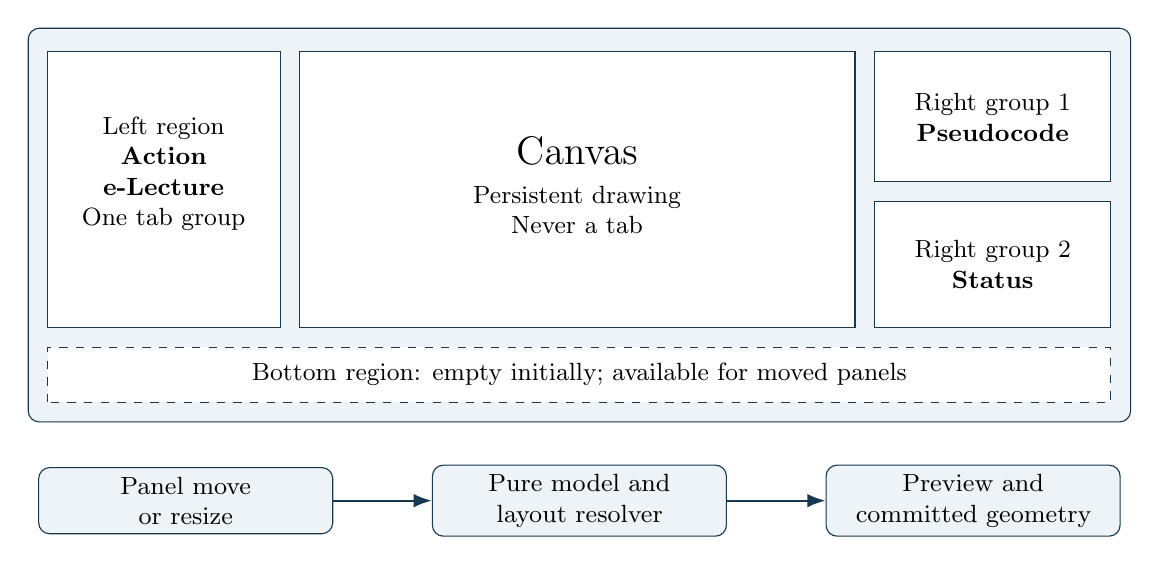
\begin{tikzpicture}[font=\small,>=Latex]
\draw[draw=navy,fill=lightblue,rounded corners] (0,0) rectangle (14,5.0);
\draw[fill=white,draw=navy] (.25,1.2) rectangle (3.2,4.7);
\node[align=center] at (1.72,3.15) {Left region\\\textbf{Action}\\\textbf{e-Lecture}\\One tab group};
\draw[fill=white,draw=navy] (3.45,1.2) rectangle (10.5,4.7);
\node[align=center] at (6.97,3.0) {\Large Canvas\\[3pt]Persistent drawing\\Never a tab};
\draw[fill=white,draw=navy] (10.75,3.05) rectangle (13.75,4.7);
\node[align=center] at (12.25,3.87) {Right group 1\\\textbf{Pseudocode}};
\draw[fill=white,draw=navy] (10.75,1.2) rectangle (13.75,2.8);
\node[align=center] at (12.25,2.0) {Right group 2\\\textbf{Status}};
\draw[fill=white,draw=navy,dashed] (.25,.25) rectangle (13.75,.95);
\node at (7,.6) {Bottom region: empty initially; available for moved panels};
\node[draw=navy,fill=lightblue,rounded corners,align=center,text width=35mm] (a) at (2,-1.0) {Panel move\\or resize};
\node[draw=navy,fill=lightblue,rounded corners,align=center,text width=35mm] (b) at (7,-1.0) {Pure model and\\layout resolver};
\node[draw=navy,fill=lightblue,rounded corners,align=center,text width=35mm] (c) at (12,-1.0) {Preview and\\committed geometry};
\draw[->,thick,navy] (a)--(b);\draw[->,thick,navy] (b)--(c);
\end{tikzpicture}
\caption{V10 layout and shared geometry calculation. The bottom region is shown as a target area; it does not reserve this height when empty.}\label{fig:v10}
\end{figure}

The main engineering decision was to express layout changes in a pure model rather than embedding all rules inside pointer-event handlers. The model preserves panel membership, removes empty groups and ensures that each group's active tab belongs to that group. Required panels occur exactly once, optional panels at most once, and groups do not nest.

A common layout resolver is used for sizing, target validity and drag previews. A proposed move is first represented in the model and then resolved into geometry, so the preview and committed result use the same constraints. Groups have minimum dimensions of 240 pixels in width and 120 pixels in height; the drawing has a target floor of 360 by 320 pixels when the viewport can accommodate it.

Saved layouts are versioned and repaired or replaced with defaults when invalid. Model tests include 4,000 seeded random operations, checks across multiple viewport sizes, and repeated serialization round trips. This validates many structural transitions, but does not replace browser testing of pointer coordinates, drag feedback and actual resizing.

\page
\subsection{The shared shell in use}
\shot{F2-dfsbfs-bfs-frame8.png}{.78}{BFS at step 8 of 22 in the default V10 arrangement. The drawing, pseudocode, status and footer transport refer to the same selected step.}{fig:bfs}
\shot{F3-tab-drag-preview.png}{.78}{Dragging the Action tab onto the Pseudocode group shows the proposed drop area. This screenshot records the preview, not a completed drop.}{fig:drag}

Figures~\ref{fig:bfs} and~\ref{fig:drag} show why layout is part of algorithm interaction. A learner may need more space for pseudocode while tracing a run, then more space for input editing. A common shell permits this adjustment without changing the underlying algorithm state. The same design is used across the three visualizer families.



\page
\subsection{Graph extensions and algorithm validation}
The current graph module contains 11 algorithm identifiers. Alongside BFS, stack-based DFS, Dijkstra, Kruskal and Edmonds--Karp, the application supports recursive DFS, Bellman--Ford, Prim, topological sorting, bipartite checking, and cut-vertex/bridge detection. Topological sorting offers DFS and Kahn methods; bipartite checking offers DFS and BFS methods. The traversal interface also supports an End node where applicable~\cite{evidence}.

These additions extend both computation and explanation. Recursive DFS exposes a different execution structure from a stack-based traversal. Topological sorting and bipartite checking provide witnesses when the input violates their conditions, rather than displaying only a final success or failure. Bellman--Ford and Prim were planned and built with Codex under my requirements and review.

\shot{F8-cut-vertex-bridge-cp4-4-7-last.png}{.90}{Final frame of cut-vertex and bridge detection on the CP4 4.7 example. The reported cut vertices are 1, 3 and 4; the bridges are 0--1 and 3--4.}{fig:cut}

\textbf{A representative correctness issue: parallel edges.} A low-link DFS must skip the parent \emph{edge}, not every edge leading to the parent vertex. If two vertices are joined by two parallel edges, removing either edge leaves them connected. Ignoring both edges during DFS can incorrectly mark one as a bridge. Stable edge identities make the intended rule explicit.

For validation, the tests compare results with independently formulated oracles. Cut vertices and bridges are checked by removing a vertex or edge and recomputing connected components. Bellman--Ford is checked against Floyd--Warshall-based results, including negative-cycle reachability. Prim is compared with exhaustive forest candidates on small inputs. These oracles are algorithmically different from the implementations under test; this reduces shared assumptions, but is not a formal proof.

The recorded randomized cases include 700 graph inputs for cut-vertex/bridge checks, 140 signed graphs for Bellman--Ford, and 20 small graphs for Prim tested from every start vertex. Topological and bipartite methods have additional randomized checks~\cite{validation}. Fixed seeds make failures reproducible. Small exhaustive cases complement, rather than replace, larger representative examples.

\page
\subsection{Tree operations and sorting comparison}
The tree visualizer provides seven workspaces: LCA, BST, AVL, Heap, Trie, Segment Tree and Lazy Segment Tree. Work includes BST/AVL queries and traversals, AVL deletion, heap operations, and lazy range-add/range-sum behaviour. The heap links array and tree representations; intermediate changes remain previews until applied. These workspaces do not imply complete operation parity with VisuAlgo~\cite{evidence}.

\shot{F6-heap-insert-climb-note.png}{.72}{Heap insertion: the new value 1 moves above 7. The array strip and tree show the same operation, with a short note explaining the comparison.}{fig:heap}

Sorting provides eight algorithms in a one-pane Study mode and two- or four-pane Compare mode. Panes share the input dataset and clock, making it possible to inspect different operation sequences on the same data. Duplicate algorithm selection is prevented and randomized quicksort uses a reproducible seed.

\shot{F7-sorting-compare-4-panes.png}{.72}{Four-pane comparison of Merge, Bubble, Quick and Radix sort on the same 48-element input. The shared operation index is a playback coordinate, not a measurement of relative runtime.}{fig:sorting}



\page
\subsection{Floating text: explanations on the canvas}\label{sec:notes}
A step can be meaningful even when the drawing hardly changes. For example, Dijkstra may reject a relaxation because the existing distance is already smaller. If the reason appears only in a separate Status panel, the learner must repeatedly look away from the relevant edge. Following the Week 10 trial, I introduced floating text: short explanations beside the relevant node or edge~\cite{evidence,architecture}. This was an important post-trial UI/UX update, intended to minimize how often users need to look at Status while following visualization steps and keep their attention on the canvas. It follows Prof.\ Halim's canvas-focused educational goal, as recalled in our project discussions. Status remains available for persistent detail; reduced attention switching is a design aim, not a measured result.

\shot{F4-sssp-dijkstra-frame24-note.png}{.94}{Dijkstra relaxation from B to E: the note explains that $4+3<8$, so E's distance changes from 8 to 7.}{fig:notes}

The implementation has a shared note description, placement calculation, timing logic and rendering layer. Graph and tree algorithms supply the semantic content; the shared layer controls how it is displayed. Current coverage includes Dijkstra, LCA, BST, AVL and Heap. Sorting, Trie, segment trees and the other graph algorithms do not yet use this layer.

Notes are rendered outside the graph transform so their text remains at a constant screen size while the anchor follows the relevant node or edge. Placement checks nearby obstacles, including node badges and edge-weight labels. It first tries preferred positions, then alternatives; when none is clear, it uses a minimum-overlap fallback. Dense graphs can therefore still produce overlap.

Timing adapts to playback. A manually inspected note normally lasts 1,600 milliseconds. During autoplay, its duration is limited by the step interval and configured delay; notes are suppressed for intervals below 200 milliseconds. This avoids accumulating unreadable text at high speed.

The note layer is currently hidden from accessibility APIs, and the application has not undergone a systematic accessibility evaluation. Future work should check whether the persistent equivalent text is sufficient and whether users can understand rejected actions, rapid transitions and dense cases without relying on colour or motion alone.

\page
\section{Current Results and Validation}\label{sec:results}
The audited build provides one site with runnable graph, tree and sorting modules. Of the 30 catalogue cards, 12 open a module; eight are labelled full and four partial in the catalogue audit, while 18 remain coming soon.~\cite{validation}.



\begin{table}[tbp]\centering\small
\caption{Recorded checks on 1 November 2026 at application commit \code{662e7b3}.}\label{tab:tests}
\begin{tabularx}{\linewidth}{@{}XrX@{}}\toprule
Check & Result & Interpretation\\\midrule
Graph unit tests & 654 passed & Algorithms, state and graph behaviour.\\
Tree unit tests & 1,881 passed & Operations, state and presentation.\\
Sorting unit tests & 571 passed & Operation streams and playback.\\
Shared / site unit tests & 143 / 24 passed & Common components and site logic.\\
\textbf{Total unit tests} & \textbf{3,273 passed} & Recorded suite total.\\
Browser cases & 151 passed & 14 specifications in Chromium.\\
Type check / build & Passed & Compile-time and production build checks.\\
Lint & 0 errors & Two warnings remained.\\\bottomrule
\end{tabularx}
\end{table}

The recorded environment was Windows 11, Node 24.17.0, npm 11.13 and Playwright 1.64.1 with Chromium. The build emitted a large-chunk warning (approximately 705 kB before gzip and 206 kB after gzip for the reported chunk).

Passing tests support regression confidence within the tested cases. They do not measure usability, accessibility, browser portability or learning.

\page
\section{User Evaluation, Limitations and Next Steps}
\subsection{Week 10 formative user trial}
In Week 10, Kerk and I invited several users to use VisuAlgo+ V10 independently for 15--20 minutes. We recorded their interactions on video, administered a short test afterwards and collected feedback. Participants varied in prior use of VisuAlgo.net, from frequent to infrequent users, and in algorithm experience, from experienced competitive programmers to beginners.

The sessions yielded positive feedback as well as areas needing improvement. Reviewing the recordings helped us identify interactions that supported familiarization with the new interface and places needing refinement. This informed subsequent UI/UX work, including floating text to keep explanations close to the visualization (Section~\ref{sec:notes}). The trial was separate from Kerk's earlier V2/V7 survey and the subsequent joint decision to adopt V10.

\subsection{Evidence boundaries and implementation limits}
The session videos, test responses and feedback have not yet been analysed, so participant numbers, scores and detailed findings are not reported here. The trial provides formative design input; a post-use test alone does not establish learning gains or comparative usability. The effect of floating text has not been measured. Performance benchmarks and a test-coverage percentage are also unavailable.

Several implementation limits are material. Graph and tree runs build eager timelines. Sorting retains unbounded history and replays operations when seeking. Step notes cover only selected algorithms and may overlap in dense drawings. Browser validation is concentrated on desktop Chromium; mobile behaviour, cross-browser compatibility and accessibility remain incomplete.

The separate engine is also a scope boundary. My unmerged engine experiment explored stable edge identity and a reusable browser client for worker/RPC lifecycle management. It helped identify integration requirements, but is not part of the deployed visualizer path.

\subsection{Proposed follow-up evaluation}
First organize the Week 10 footage, test responses and feedback into anonymized observations linked to design changes. Then conduct a more structured follow-up, provisionally involving 6--10 students familiar with introductory data structures. The participant plan and arrangements should be discussed with the supervisor before recruitment.

\begin{table}[tbp]\small\centering
\caption{Proposed follow-up tasks; these are not a reconstruction of the Week 10 test.}
\begin{tabularx}{\linewidth}{@{}p{41mm}X@{}}\toprule
Task & Evidence to collect\\\midrule
Explain a Dijkstra relaxation & Correct explanation of an accepted and rejected update; use of notes, pseudocode and Status.\\
Trace heap insertion & Correct prediction of the next swap and understanding of preview versus Apply.\\
Rearrange the workspace & Successful tab move/split, recovery from an unwanted layout, errors and assistance needed.\\
Compare two sorting runs & Ability to explain an operation difference without treating operation index as elapsed runtime.\\\bottomrule
\end{tabularx}
\end{table}

Record task completion, time, errors, requests for help and short participant comments. If a comparison with original VisuAlgo is feasible, use matched tasks and inputs and counterbalance the order. Report task-specific observations and uncertainty, rather than a single unsupported ``better UI'' conclusion.

\subsection{Proposed technical measurements}
Use a fixed machine and production build with saved inputs of increasing size. Measure run preparation, time to first visible step, seek latency, playback frame pacing and memory use. Repeat each condition at least five times and report the median together with the spread and environment. These measurements should guide whether checkpointing, bounded history or a different execution boundary is necessary.

\page
\section{Plan for the Remaining Project}
The following plan is proposed for discussion with the supervisor and Kerk. The priority is to strengthen a coherent subset of the platform before expanding the catalogue.

\begin{table}[tbp]\small\centering
\caption{Proposed milestones and completion evidence.}\label{tab:plan}
\begin{tabularx}{\linewidth}{@{}p{20mm}p{48mm}X@{}}\toprule
Window & Main work & Completion evidence\\\midrule
Nov--Dec 2026 & Consolidate Week 10 findings; stabilize the build; define follow-up tasks and automate panel interactions. & Reproducible baseline, browser tests for move/split/cancel/restore, and reviewed evaluation protocol.\\
January 2027 & Investigate one engine integration slice with Kerk, starting with a simple graph algorithm. & Written input/step contract; matching results and playback semantics against the TypeScript reference.\\
February & Conduct follow-up task evaluation and technical measurements. & Anonymized observations, fixed benchmark inputs, environment and result tables.\\
March & Address high-impact findings; improve explanation and accessibility for selected modules. & Before/after regression checks and follow-up verification of the changed tasks.\\
April & Consolidate results, document limitations, and prepare the final report and demonstration. & Reproducible release snapshot, final evaluation account and presentation materials.\\\bottomrule
\end{tabularx}
\end{table}

\subsection{Integration strategy and risks}
Engine integration should begin with one vertical slice: graph input, engine execution, typed step conversion, rendering and backward/forward playback. The first milestone is behavioural agreement, including edge identities and cancellation, rather than replacing every TypeScript algorithm. If the engine contract or schedule is not ready, the existing implementation remains a functional baseline and the report can document the integration study separately.

The main technical risks are the cost of long timelines, inconsistent semantics between modules, and interaction failures that model tests do not expose. Measurements should precede a major playback redesign. Shared abstractions should be introduced only where behaviour is truly common; graph/tree eager sequences and sorting generators already demonstrate that identical controls need not imply identical execution internals.

The main project risk is scope growth. Adding every unfinished catalogue topic would reduce time for evaluation and refinement. I propose prioritizing the current graph, tree and sorting workflows, selected explanation gaps and a small engine experiment. Further features should be chosen with the supervisor according to educational value, missing coverage and available time.

\subsection{Expected outcome}
By the final assessment, the intended outcome is a documented and tested visualization foundation with a coherent interface, representative algorithm coverage, evidence from user tasks and technical measurements, and a clear account of engine integration progress. The first-semester work establishes the implementation base. The next phase should explain where it works well, where it fails, and which improvements are supported by evidence.

\page
\begingroup
\small
\setlength{\parskip}{3pt}
\bibliographystyle{plain}
\bibliography{references}
\endgroup
\end{document}
